% workaround for problem with white text if notes are enabled
% http://tex.stackexchange.com/questions/232168/normal-text-is-invisible-when-using-beamer-with-notes-and-xelatex
\def\pgfsysdriver{pgfsys-dvipdfm.def}

\documentclass{beamer}

\usetheme{metropolis}
\setbeamercolor{normal text}{bg=white} % white background instead of black!2


% colors from metropolis
\colorlet{codeString}{mLightGreen}
\colorlet{codeKeyword}{mLightBrown}

\usepackage{pgfpages}
\setbeameroption{show notes on second screen}


\usepackage{ifxetex}
\ifxetex
  \usepackage{polyglossia}
  \setmainlanguage{russian}
  \setotherlanguage{english}

  % workaround for "Package polyglossia Error: The current roman font does not contain the Cyrillic script!"
  \newfontfamily\cyrillicfonttt{Fira Mono}
\else
  \usepackage[T2A]{fontenc}
  \usepackage[utf8]{inputenc}
  \usepackage[english,russian]{babel}

  % workaround for "Package hyperref Warning: Glyph not defined in PD1 encoding"
  \hypersetup{unicode=true}
\fi

\newcommand{\eng}[1]{%
  \ifxetex%
    {\textenglish{#1}}%
  \else%
    {\foreignlanguage{english}{#1}}%
  \fi%
}

\usepackage{listings}
\lstset{
  basicstyle=\ttfamily,
  keywordstyle=\bfseries\color{codeKeyword},
  stringstyle=\color{codeString},
  showstringspaces=false
}

% numbers formating: \num{123456}
\usepackage{numprint}
\newcommand{\num}[1]{\numprint{#1}}
  \npthousandsep{\,}
  \npthousandthpartsep{}
  \npdecimalsign{,}

\newcommand{\pcnum}[1]{\ensuremath{\mathtt{#1}}}
\newcommand{\bin}[1]{\pcnum{#1}_2}
\newcommand{\hex}[1]{\pcnum{#1}_{16}}

\newcommand{\code}[1]{\texttt{#1}}

\hypersetup{pdfauthor={Владимир Парфиненко}}
\title{Основы программирования}
\subtitle{Лекция № 2, XX февраля 2016 г.}
\date{}
\institute{
  \vspace{1em}
  \centering
  \parbox{0.8\textwidth}{
    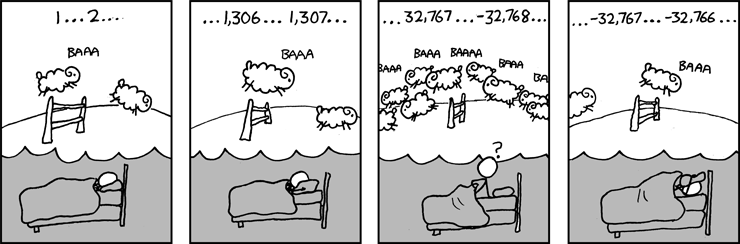
\includegraphics[width=\linewidth]{xkcd_cant_sleep}
    \par
    \raggedleft\tiny\url{http://xkcd.com/571}
  }
}


\begin{document}

\begin{frame}[plain]
  \titlepage
\end{frame}

\begin{frame}{Знакомство}

  Я~--- Владимир Парфиненко,

  \begin{itemize}
    \item бакалавр физики (ФФ), магистр математики (ММФ),
    \item профессиональный программист (Excelsior),
    \item регулярно чему-то учу (ФФ, АФТИ, ЛШ ФМШ).
  \end{itemize}

  Контакт:
  \href{mailto:vladimir.parfinenko@gmail.com}{vladimir.parfinenko@gmail.com}

\end{frame}

\section{Представление целых чисел}
\note{
  Порассуждать о том, как с помощью двух ламп можно представить числа от 0 до 3
}

\begin{frame}{Двоичная система счисления}

  Самый простой метод записи чисел, использующий только две цифры: 0 и 1.
  \note{компьютеру легко работать с такими числами\\}

  С помощью $n$ \emph{позиций} можно записать $2^n$ чисел.
  \note{Суффикс $x_{10}$ будем опускать\\}
  \begin{align*}
    \bin{000} &= 0, &\qquad \bin{100} &= 4, \\
    \bin{001} &= 1, &\qquad \bin{101} &= 5, \\
    \bin{010} &= 2, &\qquad \bin{110} &= 6, \\
    \bin{011} &= 3, &\qquad \bin{111} &= 7.
  \end{align*}
\end{frame}

\begin{frame}{Двоичная система счисления}

  Перевод из двоичной в десятичную:
  \[
    \bin{11001} = \mathbf{1} \cdot 2^4 + \mathbf{1} \cdot 2^3 +
                  \mathbf{0} \cdot 2^2 + \mathbf{0} \cdot 2^1 +
                  \mathbf{1} \cdot 2^0 = 16 + 8 + 1 = 25.
  \]
  Перевод из десятичной в двоичную:
  \note{сказать про обратный порядок\\}
  \begin{align*}
    25 &= 2 \cdot 12 + \mathbf{1}, \\
    12 &= 2 \cdot 6 + \mathbf{0}, \\
    6 &= 2 \cdot 3 + \mathbf{0}, \\
    3 &= 2 \cdot 1 + \mathbf{1}, \\
    1 &= 2 \cdot 0 + \mathbf{1}.
  \end{align*}

\end{frame}

\begin{frame}{Числа в памяти компьютера}

  1 \emph{байт} состоит из 8 \emph{бит} и может кодировать $2^8 = 256$
  различных чисел.
  \note{пояснить, что байт - минимальная ячейка памяти, которую компьютер может
  читать/писать\\}

  Например, число 337 кодируется минимум 2 байтами:
  \[
    \underbrace{\pcnum{00000001}}_{\text{биты } 15 \ldots 8}
    \underbrace{\pcnum{01010001}}_{\text{биты } 7 \ldots 0}
  \]

  Предельные значения:
  \begin{itemize}
    \item 8 бит: $0 \ldots \num{255}$,
    \item 16 бит: $0 \ldots \num{65535}$,
    \item 32 бита: $0 \ldots \num{4294967295}$,
    \item 64 бита: $0 \ldots \num{18446744073709551615}$.
  \end{itemize}
\end{frame}

\begin{frame}{Шестнадцатеричная система счисления}

  Цифры: $\pcnum{0}, \pcnum{1}, \pcnum{2}, \pcnum{3}, \pcnum{4}, \pcnum{5},
  \pcnum{6}, \pcnum{7}, \pcnum{8}, \pcnum{9}, \pcnum{A}, \pcnum{B}, \pcnum{C},
  \pcnum{D}, \pcnum{E}, \pcnum{F}$.

  Перевод в двоичную и обратно через тетрады (по 4 бита):
  \[
    \bin{101011100} = \pcnum{\{0001\}\{0101\}\{1100\}} = \hex{15C}.
  \]

  «Понятная» запись констант:
  \begin{itemize}
    \item 8 бит: диапазон чисел $\hex{0} \ldots \hex{FF}$,
    \item 32 бита: диапазон чисел $\hex{0} \ldots \hex{FFFFFFFF}$,
    \item $\texttt{0xDEADBEEF}, \texttt{0xCAFEBABE}, \texttt{0xCDCDCDCD},
      \ldots$
      \note{отладочная печать, Java-класс файл, неинициализированная память\\}
  \end{itemize}

\end{frame}

\begin{frame}{Знаковые числа}

  \note[item]{
  Отдельной памяти под знак нет, поэтому нужно упаковывать его в те же 8 (16,
  32, \ldots) бит.
  }

  \note[item]{
  Заметим, что компьютер выполняет сложение и вычитание по модулю,
  соответствующему размеру числа.
  }

  Рассмотрим сложение двух 8-битных чисел
  $\hex{FF} + \hex{01}$:
  \[
    \begin{array}{r}
    +
      \begin{array}{r}
        \pcnum{11111111} \\
        \pcnum{00000001} \\
      \end{array} \\
      \hline
      \begin{array}{r}
        \pcnum{1}\underbrace{\pcnum{00000000}}_{8 \text{ бит}}
      \end{array}
    \end{array}
  \]

  С точки зрения компьютера $(\hex{FF} + \hex{01}) \mod 2^8 = \hex{00}$.

  То есть $X + 1 = 0$. Чему равно $X$?

\end{frame}

\begin{frame}{Знаковые числа}

  Для представления отрицательных чисел используется \emph{двоичный
  дополнительный код}:
  \[ -X = 2^N - X, \text{где $N$~--- размер числа.}\]

  8-битные знаковые числа:
  \begin{align*}
    \bin{0000 0000} &= 0,    &\qquad \bin{1000 0000} &= -128, \\
    \bin{0000 0001} &= 1,    &\qquad \bin{1000 0001} &= -127, \\
                    &\ldots, &\qquad                 &\ldots, \\
    \bin{0111 1110} &= 126,  &\qquad \bin{1111 1110} &= -2,   \\
    \bin{0111 1111} &= 127,  &\qquad \bin{1111 1111} &= -1.
  \end{align*}

  \note{Сложение и вычитание не отличается от беззнаковых чисел.\par}
  \note{Умножение и деление~--- специфичное.\par}

\end{frame}

\begin{frame}{Переполнение}

  Беззнаковые 8-битные:
  \begin{itemize}
    \item $255 + 1 = \bin{1111 1111} + 1 = \bin{0000 0000} = 0$,
    \item $0 - 1 = \bin{0000 0000} - 1 = \bin{1111 1111} = 255$.
  \end{itemize}

  Знаковые 8-битные:
  \begin{itemize}
    \item $127 + 1 = \bin{0111 1111} + 1 = \bin{1000 0000} = -128$,
    \item $-128 - 1 = \bin{1000 0000} - 1 = \bin{0111 1111} = 127$.
  \end{itemize}

\end{frame}

\begin{frame}{\eng{Epic Fails}}

  \begin{itemize}
    \item 22 сентября 2009 г.~--- \eng{Twitter}: порядковый номер твитов
      переполнил 32-битное беззнаковое целое.

    \item 9 февраля 2013 г.~--- \eng{OpenStreetMap}: порядковый номер точек на
      карте переполнил 32-битное знаковое целое.

    \item 1 декабря 2014 г.~--- \eng{YouTube}: количество просмотров
      \href{https://www.youtube.com/watch?v=9bZkp7q19f0}{одного видео}
      переполнило 32-битное знаковое целое.
  \end{itemize}

  \note{В абсолютном большинстве случаев хватит 32-битных чисел.\par}

\end{frame}

\section{Целочисленные типы данных в C и~операции над ними}

\begin{frame}{Беззнаковые целочисленные типы в C}

  \begin{table}
    \begin{tabular}{ccc}
      \hline
      Тип              & Размер, бит & Максимум  \\
      \hline
      \code{unsigned char}      & 8  & $\num{255}$ \\
      \code{unsigned short}     & 16 & $\num{65535}$ \\
      \code{unsigned int}       & 32 & $\num{4294967295}$ \\
      \code{unsigned long long} & 64 & $\num{18.4e18}$ \\
      \hline
    \end{tabular}
  \end{table}

\end{frame}

\begin{frame}{Знаковые целочисленные типы в C}

  \begin{table}
    \begin{tabular}{ccrl}
      \hline
      Тип              & Размер, бит & Минимум             & Максимум  \\
      \hline
      \code{signed char}        & 8  & $\num{-128}$        & $\num{127}$ \\
      \code{short}              & 16 & $\num{-32768}$      & $\num{32767}$ \\
      \code{int}                & 32 & $\num{-2147483648}$ & $\num{2147483647}$ \\
      \code{long long}          & 64 & $\num{-9.2e18}$     & $\num{9.2e18}$ \\
      \hline
    \end{tabular}
  \end{table}

\end{frame}

\begin{frame}{Арифметические операции}

  \begin{table}
    \begin{tabular}{cc}
      \hline
      Оператор      & Операция \\
      \hline
      \code{a + b}  & сложение \\
      \code{a - b}  & вычитание \\
      \code{a / b}  & деление нацело \\
      \code{a \% b} & остаток от деления \\
      \code{-a}     & отрицание \\
      \code{a++}    & инкремент \\
      \code{a--}    & декремент \\
      \hline
    \end{tabular}
  \end{table}

\end{frame}


\defverbatim[colored]\lstAbs{
\begin{lstlisting}[language=C]
    int x;
    printf("Enter number: ");
    scanf("%d", &x);
    if (x < 0) {
        x = -x;
    }
    printf("Absolute value = %d\n", x);
\end{lstlisting}
}

\defverbatim[colored]\lstAbsLogA{
\begin{lstlisting}
    Enter number: -37
    Absolute value = 37
\end{lstlisting}
}

\defverbatim[colored]\lstAbsLogB{
\begin{lstlisting}[escapeinside={/**}{**/}]
    Enter number: -2147483648
    Absolute value = -2147483648
\end{lstlisting}
}

\begin{frame}{Загадка: модуль числа неотрицательный?}

  \begin{block}{Вычисление модуля введенного числа:}
    \lstAbs
  \end{block}

  \begin{block}{Исполнение:}
    \only<1>{\lstAbsLogA}
    \only<2>{\lstAbsLogB}
  \end{block}

\end{frame}

\begin{frame}{Битовые логические операции}

  Целое число~--- это лишь набор битов.

  \begin{block}{Бинарные:}
    \[
      \text{\eng{AND} (\code{\&}):}\thickspace
      \begin{array}{r}
        \pcnum{0101} \\
        \pcnum{0011} \\
        \hline
        \pcnum{0001}
      \end{array}
      \qquad
      \text{\eng{OR} (\code{|}):}\thickspace
      \begin{array}{r}
        \pcnum{0101} \\
        \pcnum{0011} \\
        \hline
        \pcnum{0111}
      \end{array}
      \qquad
      \text{\eng{XOR} (\code{\textasciicircum}):}\thickspace
      \begin{array}{r}
        \pcnum{0101} \\
        \pcnum{0011} \\
        \hline
        \pcnum{0110}
      \end{array}
    \]
  \end{block}

  \begin{block}{Унарные:}
    \[
      \text{\eng{NOT} (\code{\textasciitilde}):}\thickspace
      \begin{array}{r}
        \pcnum{0101} \\
        \hline
        \pcnum{1010}
      \end{array}
    \]
  \end{block}

\end{frame}

\begin{frame}{Битовые сдвиги}

  TODO

\end{frame}

\section{Числа с плавающей точкой}

\plain{Конец второй лекции}

\end{document}
